%\documentclass[a4paper]{article}
\usepackage[utf8]{inputenc}
\usepackage[spanish, es-tabla, es-noshorthands]{babel}
\usepackage[table,xcdraw]{xcolor}
\usepackage[a4paper, footnotesep=1.25cm, headheight=1.25cm, top=2.54cm, left=2.54cm, bottom=2.54cm, right=2.54cm]{geometry}
%\geometry{showframe}

%\usepackage{wrapfig}			%Wrap figure in text
\usepackage[export]{adjustbox}	%Move images
\usepackage{changepage}			%Move tables

\usepackage{tikz}
\usepackage{amsmath}
\usepackage{amsfonts}
\usepackage{amssymb}
\usepackage{float}
\usepackage{graphicx}
\usepackage{caption}
\usepackage{subcaption}
\usepackage{multicol}
\usepackage{multirow}
\usepackage{wrapfig}
\setlength{\doublerulesep}{\arrayrulewidth}
\usepackage{booktabs}
\usepackage[numbib, nottoc, notlot, notlof]{tocbibind}

\usepackage{hyperref}
\hypersetup{
    colorlinks=true,
    linkcolor=blue,
    filecolor=magenta,      
    urlcolor=blue,
    citecolor=blue,    
}

%Change Font Size

% #1 = size, #2 = text
\newcommand{\setparagraphsize}[2]{{\fontsize{#1}{6}\selectfont#2 \par}}		%Cambia el size de todo el parrafo
\newcommand{\setlinesize}[2]{{\fontsize{#1}{6}\selectfont#2}}				%Cambia el font de una oración

\newcommand{\note}[1]{
	\begin{center}
		\huge{ \textcolor{red}{#1} }
	\end{center}
}

%FONTS (IMPORTANTE): Compilar en XeLaTex o LuaLaTeX
\usepackage{anyfontsize}	%Font size
\usepackage{fontspec}		%Font type

\usepackage{etoolbox}
\usepackage{todonotes}

\newcommand{\observacion}[2]{  \ifnumequal{1}{#1}{ { \todo[inline,backgroundcolor=red!25,bordercolor=red!100]{\textbf{Observación: #2}} } }{  }  }

\setcounter{topnumber}{2}
\setcounter{bottomnumber}{2}
\setcounter{totalnumber}{4}
\renewcommand{\topfraction}{0.85}
\renewcommand{\bottomfraction}{0.85}
\renewcommand{\textfraction}{0.15}
\renewcommand{\floatpagefraction}{0.8}
\renewcommand{\textfraction}{0.1}
\setlength{\floatsep}{5pt plus 2pt minus 2pt}
\setlength{\textfloatsep}{5pt plus 2pt minus 2pt}
\setlength{\intextsep}{5pt plus 2pt minus 2pt}

\newcommand{\quotes}[1]{``#1''}
\usepackage{array}
\newcolumntype{C}[1]{>{\centering\let\newline\\\arraybackslash\hspace{0pt}}m{#1}}
\usepackage[american]{circuitikz}
\usetikzlibrary{calc}
\usepackage{fancyhdr}
\usepackage{units} 

\graphicspath{{../Control de posición no lineal/}{../Control de fuerza no lineal/}{../Control híbrido no lineal/}{../Referencias/}{../Deducción de modelo/}{../Conclusiones/}}

\pagestyle{fancy}
\fancyhf{}
\lhead{22.99 - Automación Industrial}
\rhead{Lambertucci, Londero B., Maselli, Mechoulam}
\rfoot{Página \thepage}

%Items con bullets y no cuadrados
\renewcommand{\labelitemi}{\textbullet }

%
%\begin{document}

\subsection{Consideraciones previas}
Antes de comenzar el análisis es importante destacar que previo a iniciar con el proceso que se describe a continuación, se verificó la controlabilidad y observabilidad del sistema. Los resultados de esto, son que el sistema es observable cuando se toma como salida del mismo la posición del carrito. Sin embargo, no lo es tomando como salida el angulo del péndulo.

\subsection{Linealización}
En base a las Ecuaciones (\ref{eq:aym}), se linealiza el sistema en el punto de equilibrio donde todas las variables de estado son nulas. Además, se toma como salida del sistema, la posición del carrito, para poder implementar luego un observador de estados.
Se obtiene entonces el siguiente sistema en espacio de estados.
\begin{equation}
A=
	\begin{pmatrix}
		0   & 1.0000  &       0   &      0\\
         0  &       0  &  2.6727   &      0\\
         0     &   0      &   0  &  1.0000\\
         0    &     0  & 31.1818      &   0\\
	\end{pmatrix} \ \ \
B=
	\begin{pmatrix}
		 0\\
    1.8182\\
         0\\
    4.5455\\

	\end{pmatrix} \ \ \
C=
\begin{pmatrix}
		1&0&0&0

	\end{pmatrix} \ \ \
D=0
\end{equation}

Estas matrices representativas del sistema linealizado en espacio de estados, son utilizadas luego para calcular las ganancias en la realimentacion para cada uno de los estados.

\subsection{Tiempo continuo}
Para realizar el análisis es este caso se utiliza el diagrama de Simulink que se observa en la Figura (\ref{fig:onlyFeed}), colocando todos los polos del sistema en -10 con la función \textit{acker()}.
\begin{figure}[H]
	\centering
	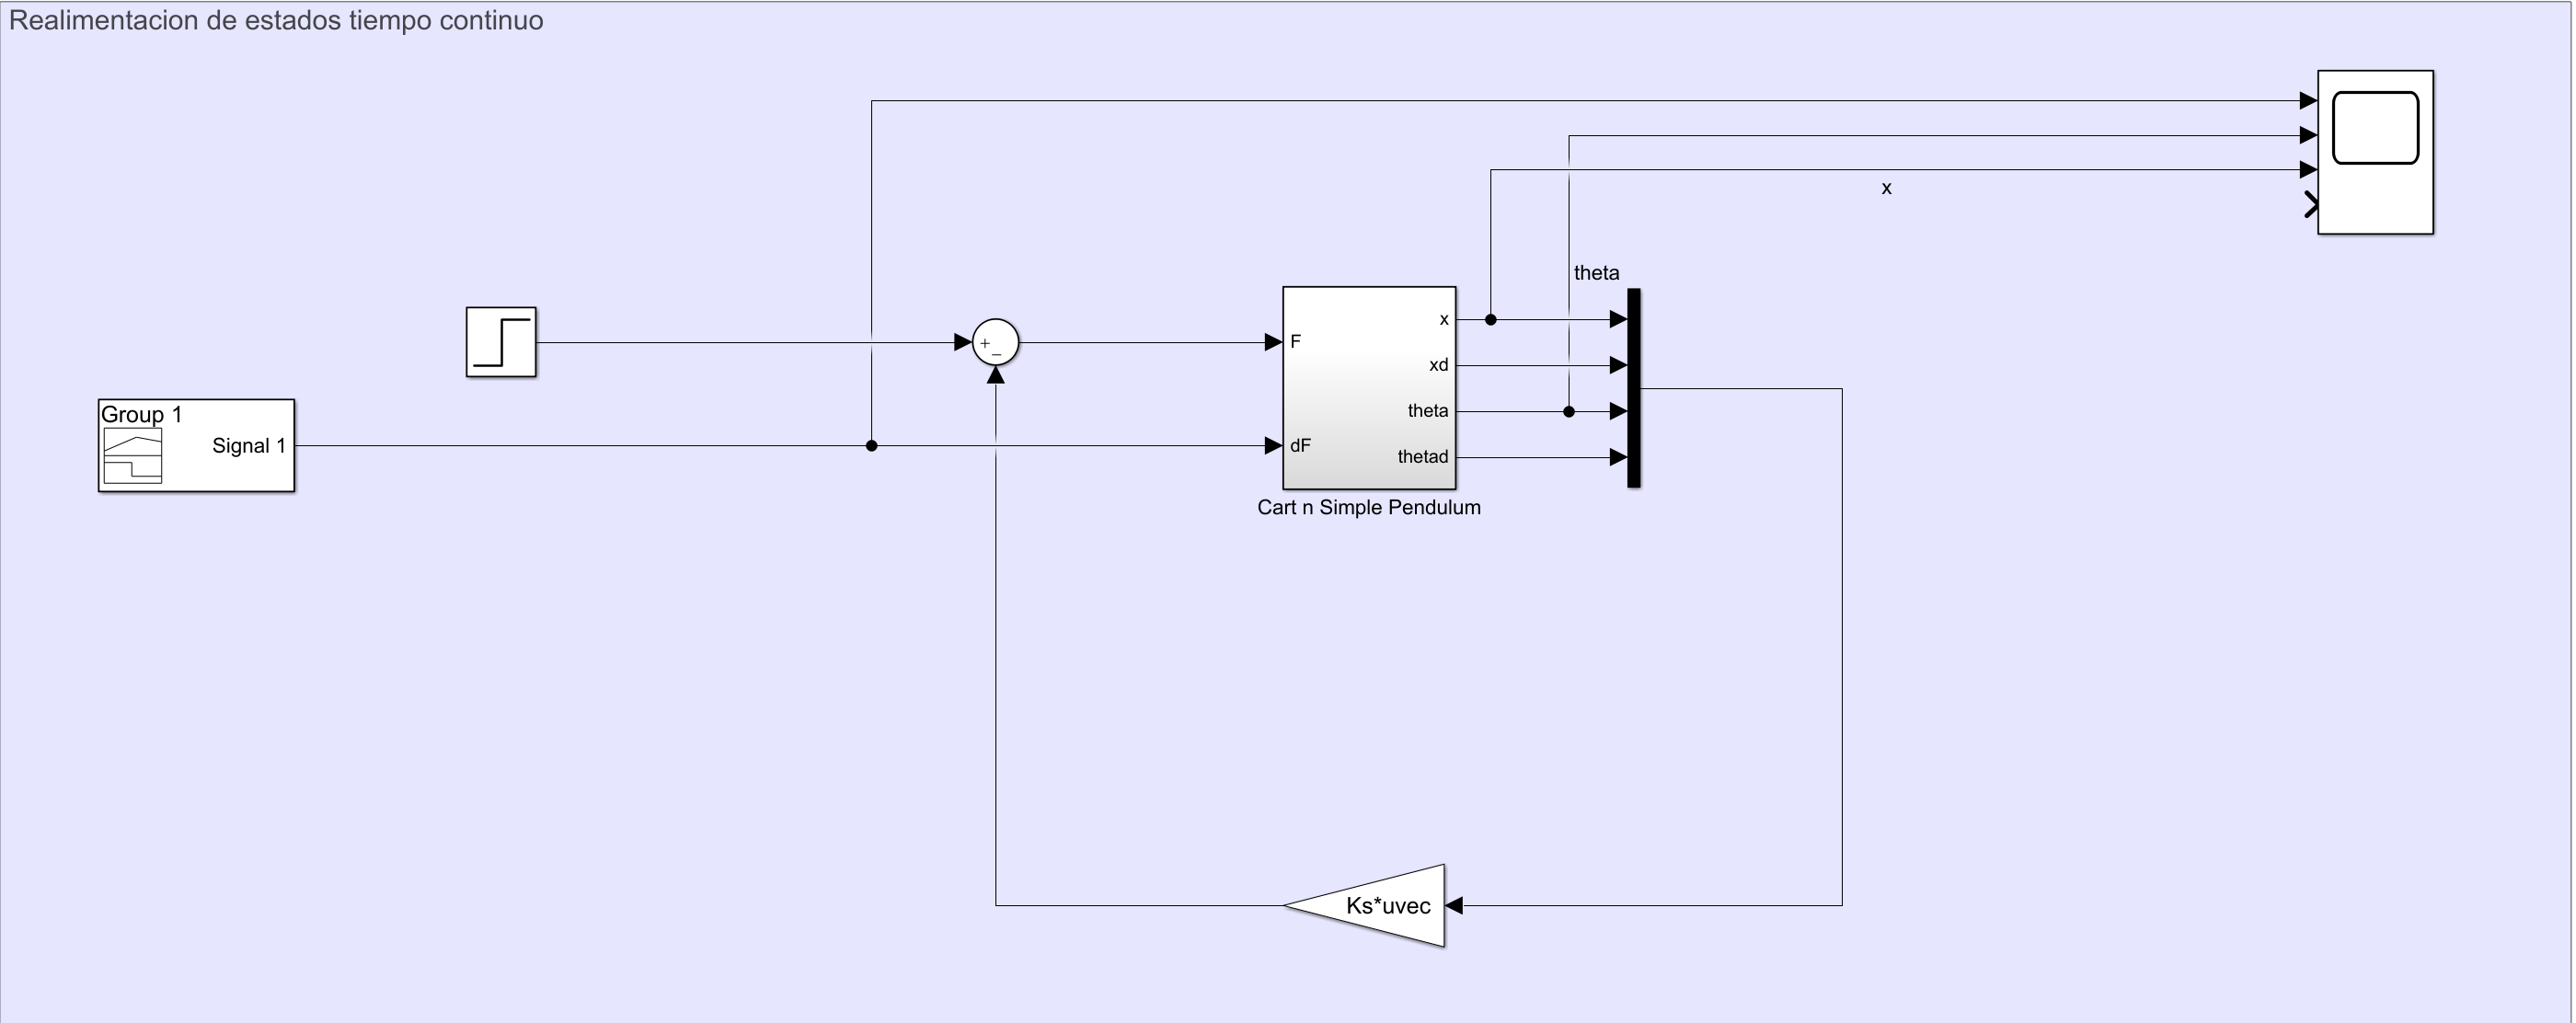
\includegraphics[width=0.8\linewidth]{ImagenesRealimentacióndeEstados/onlyFeed}
	\caption{Control por Realimentación de estados en tiempo continuo.}	
	\label{fig:onlyFeed}
\end{figure}
Se muestra en la Figura (\ref{fig:onlyFeedOut}) tanto las salidas como las entradas del sistema. Puede observarse que tanto al aplicar el escalón inicial de fuerza como al aplicar un disturbio a los 4 segundos, el sistema es capaz de retornar a la posición de equilibrio en un tiempo menor a 3 segundos para el caso de la mayor perturbación.

Se observa además, que el sistema tiene error permanente en la posición del carrito, es por ello que se impementa a continuación la acción integral.
\begin{figure}[H]
	\centering
	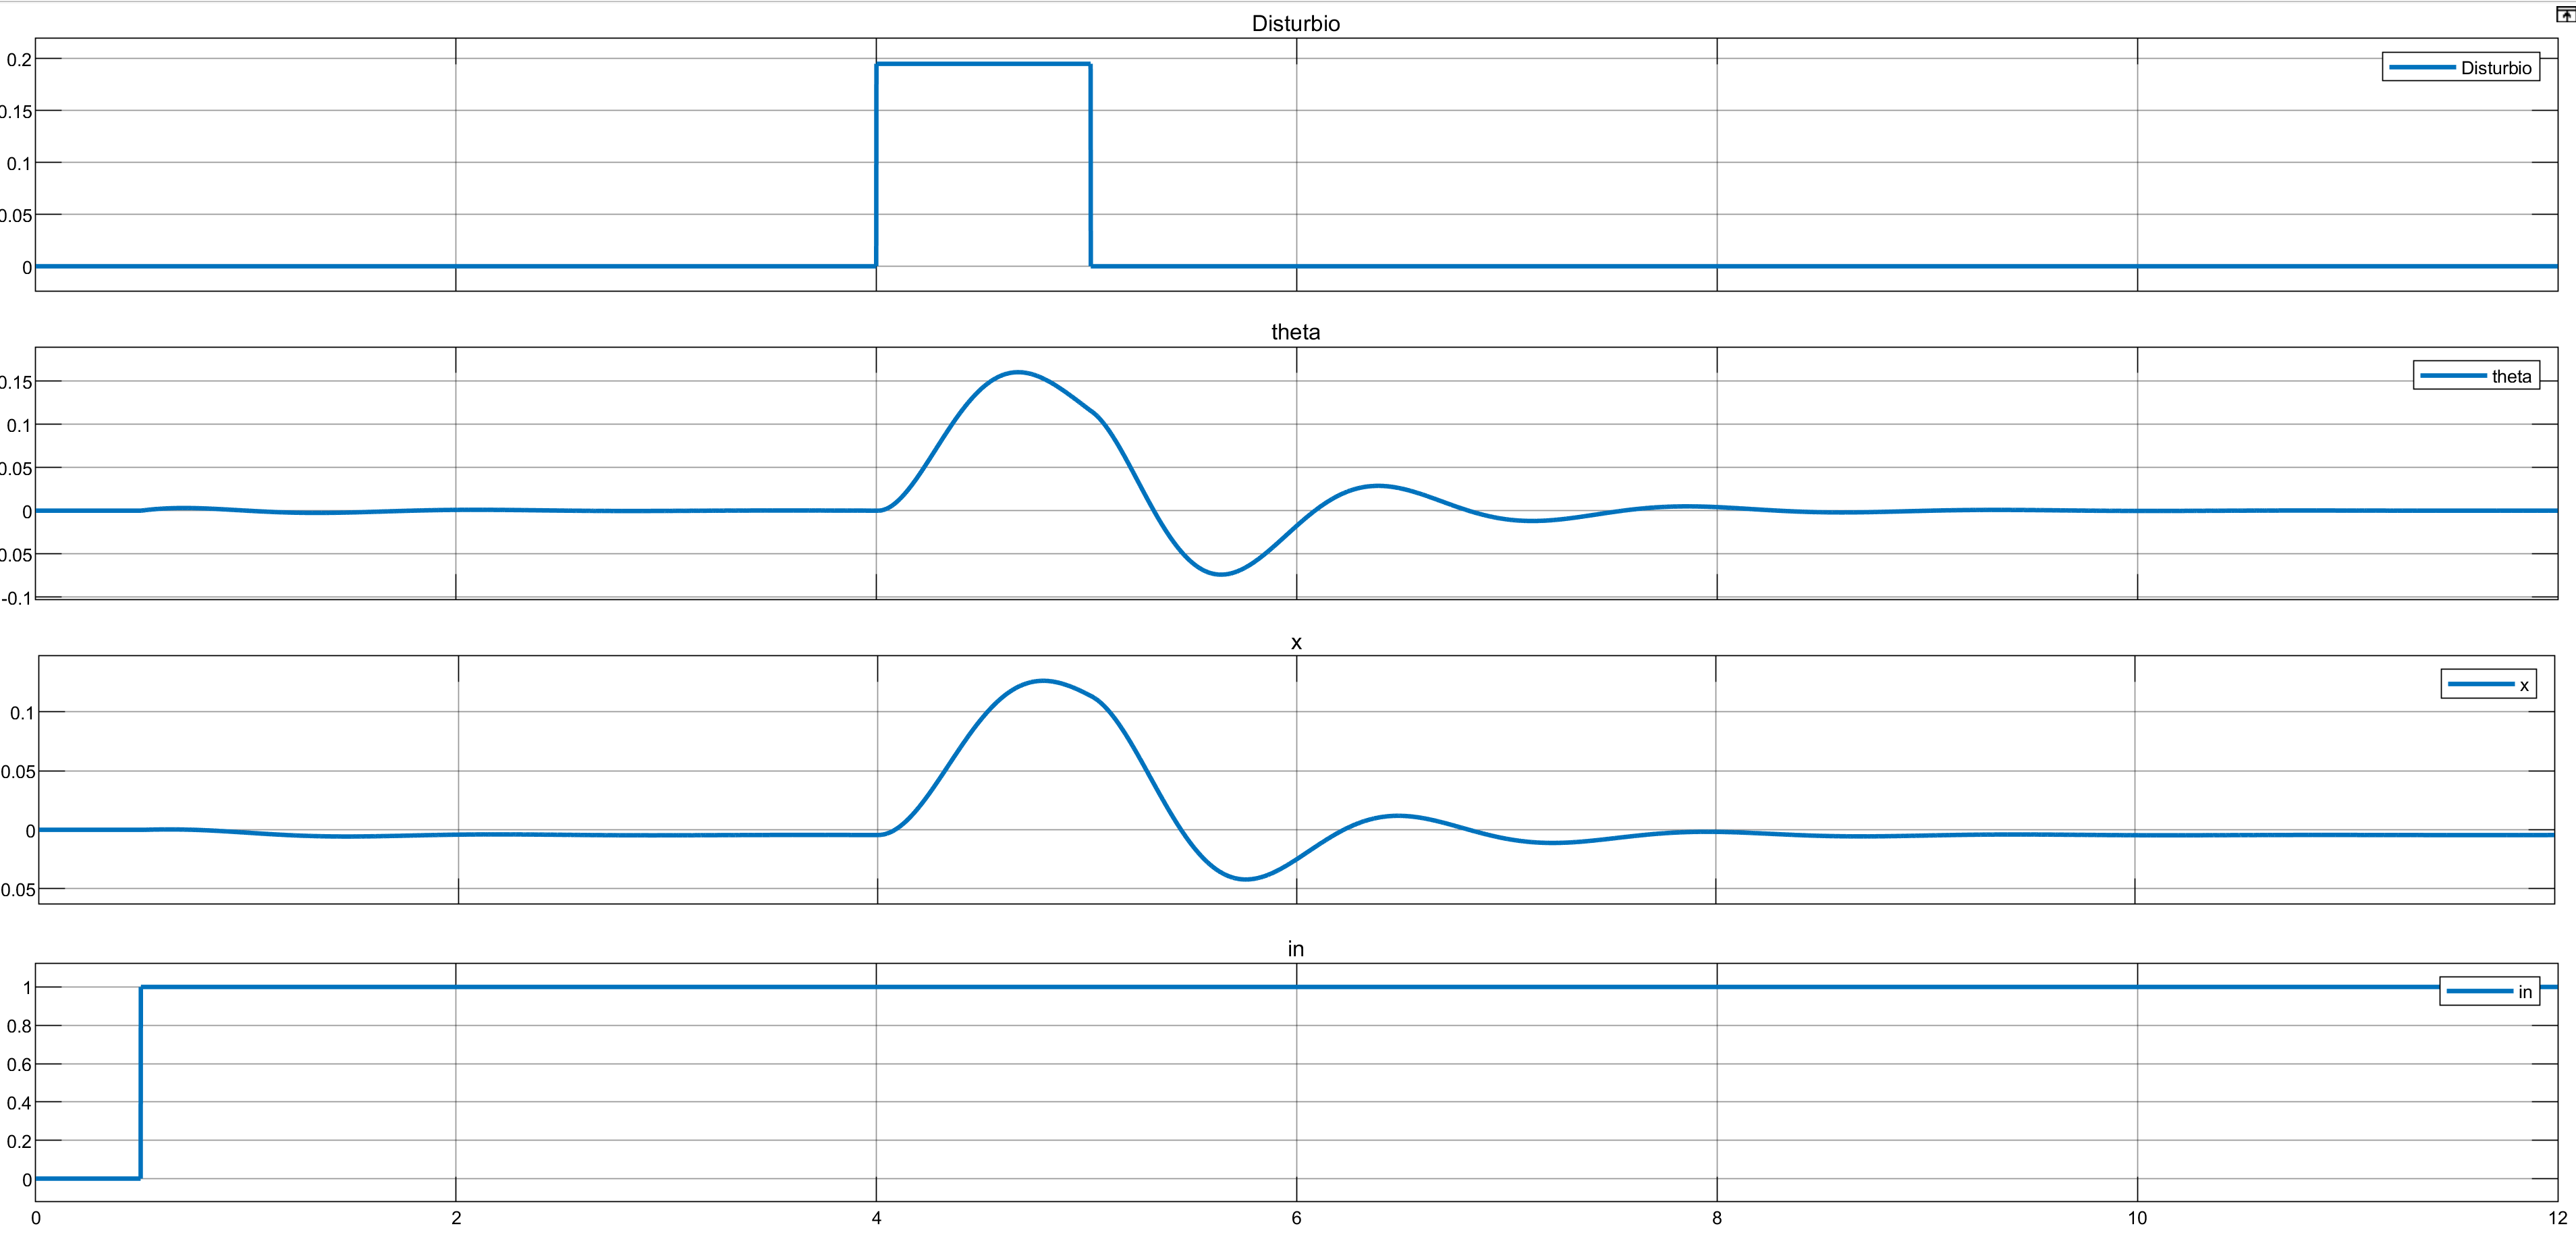
\includegraphics[width=0.8\linewidth]{ImagenesRealimentacióndeEstados/onlyFeedOut}
	\caption{Salidas y entradas del control por realimentaci\'on de estados en tiempo continuo}	
	\label{fig:onlyFeedOut}
\end{figure}

\subsection{Control integral en tiempo continuo}
Con el fin de eliminar el error permanente, se implementa el sistema con acción integral como se ve en la Figura (\ref{fig:integralFeed}). Cabe aclarar que se le agrega la posibilidad de cambiar la referencia del sistema, pudiendo así seleccionar la posición final del carrito respeto al origen.
\begin{figure}[H]
	\centering
	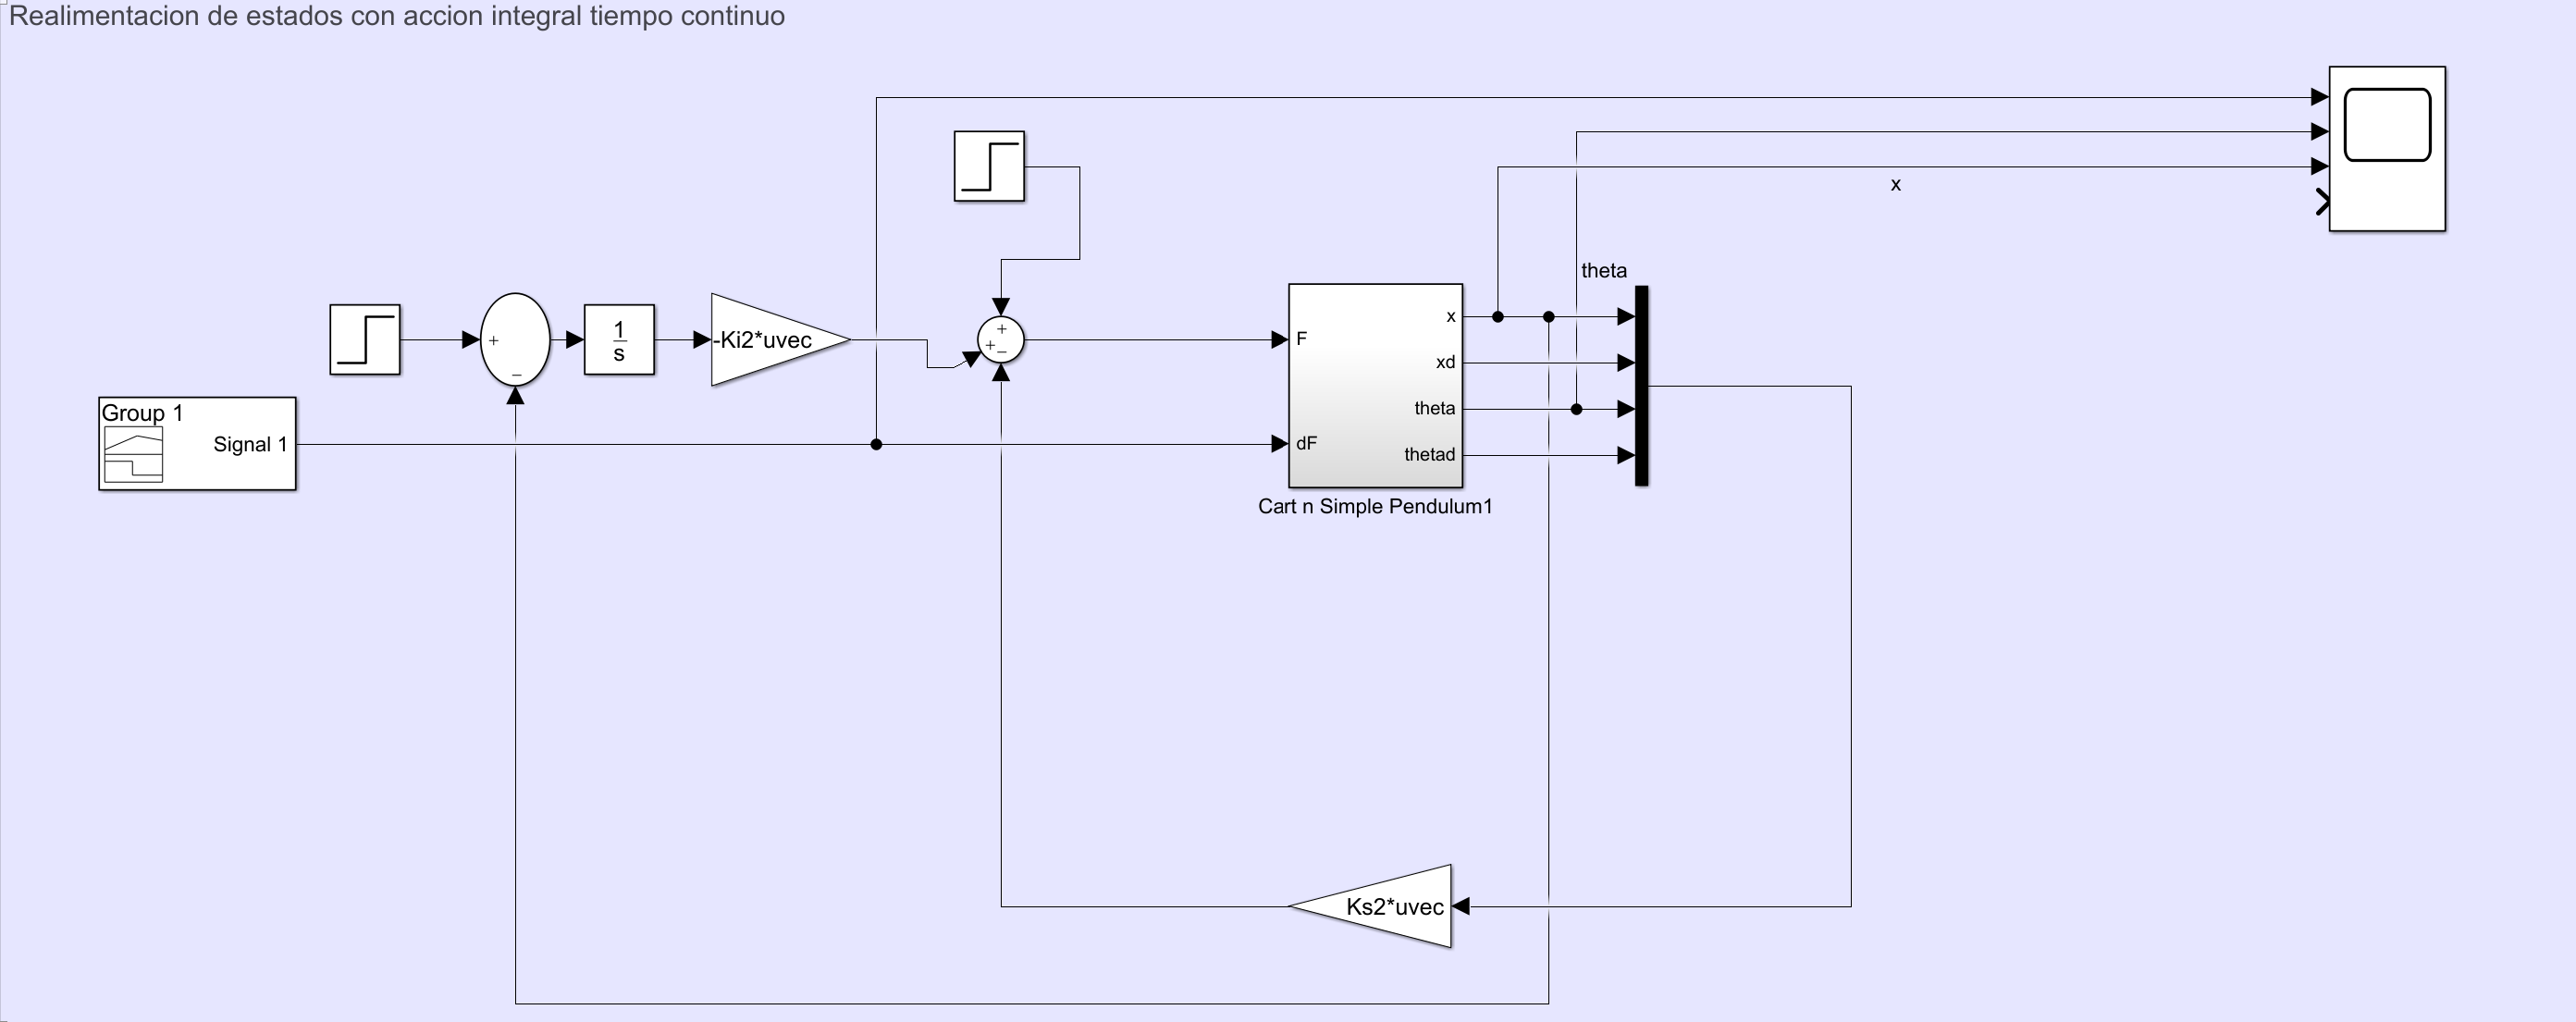
\includegraphics[width=0.8\linewidth]{ImagenesRealimentacióndeEstados/integralFeed}
	\caption{Control por Realimentación de estados con acción integral en tiempo continuo.}	
	\label{fig:integralFeed}
\end{figure}

Los polos del sistema se ubican teniendo cuidado de colocar 2 polos lentos relacionados con las variables de posición y velocidad de carrito y 2 polos mas rápidos relacionados con el angulo y la velocidad angular del péndulo, siendo así estos ubicados en -3 y -15 respectivamente. 

\begin{figure}[H]
	\centering
	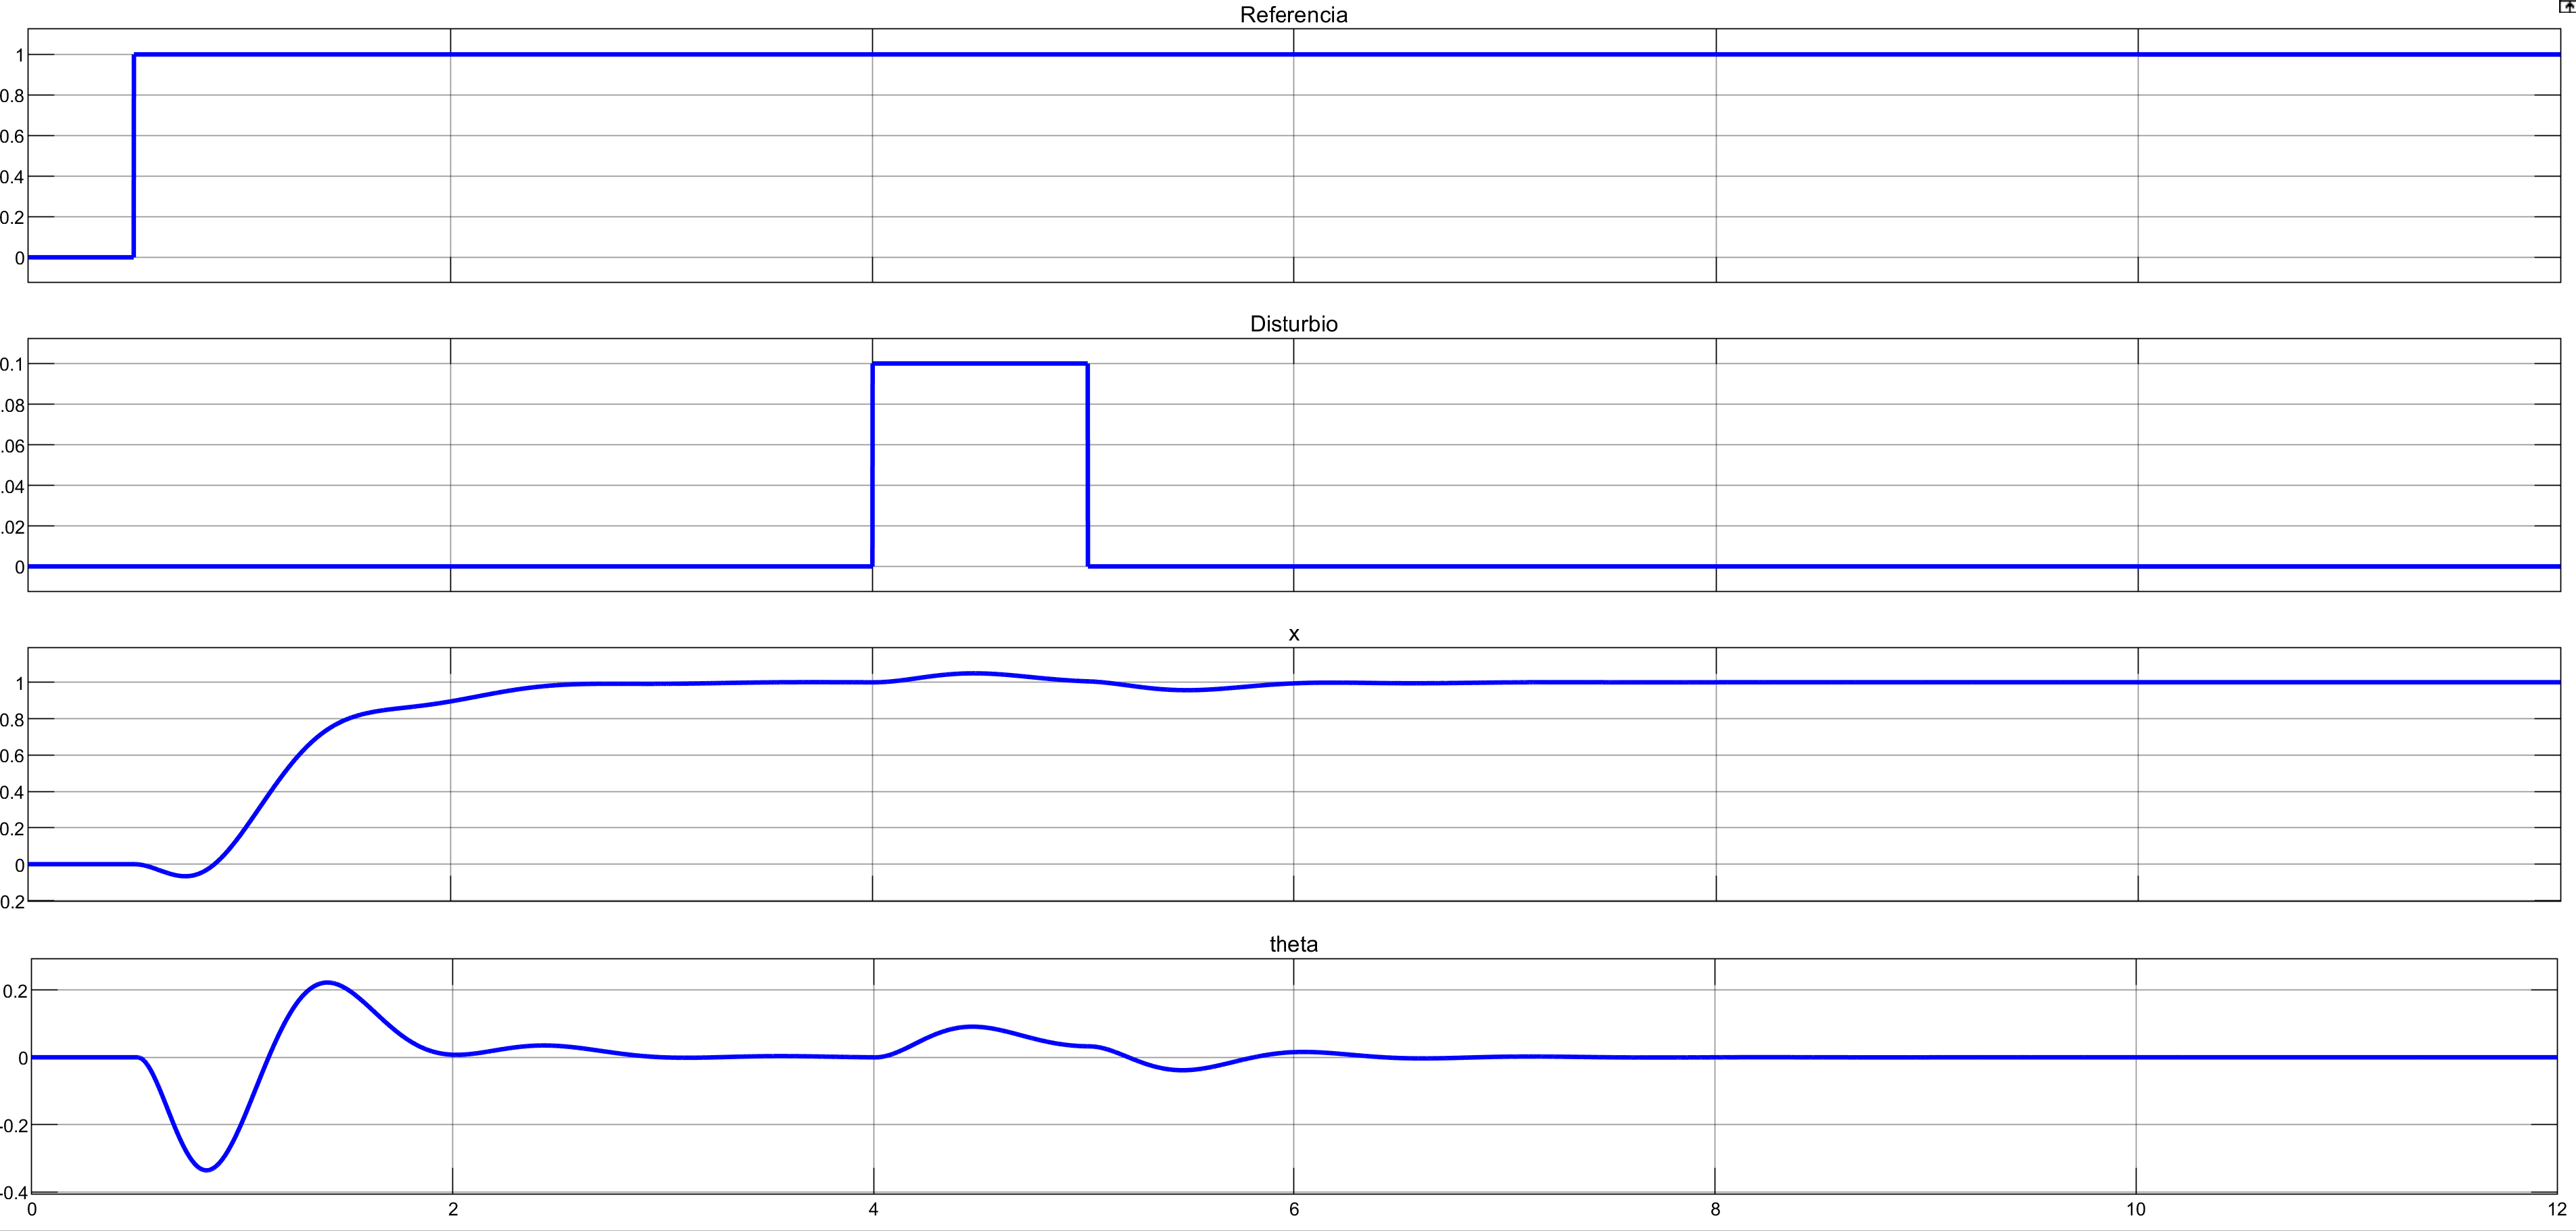
\includegraphics[width=0.8\linewidth]{ImagenesRealimentacióndeEstados/integralFeedOut}
	\caption{Entradas y salidas del Control por Realimentación de estados con acción integral en tiempo continuo.}	
	\label{fig:integralFeedOut}
\end{figure}

En la Figura (\ref{fig:integralFeedOut}) se observa que el sistema se estabiliza rápidamente tanto al cambiar la referencia como ante un disturbio y en este caso se logra eliminar el error permanente.

\subsection{Control integral en tiempo discreto}
Por último se implementa el sistema con acción integral en tiempo discreto, utilizando un integrador discreto y los \textit{Zero Orer Hold} correspondientes, como e observa en la Figura (\ref{fig:discreteIntegralFeed})
\begin{figure}[H]
	\centering
	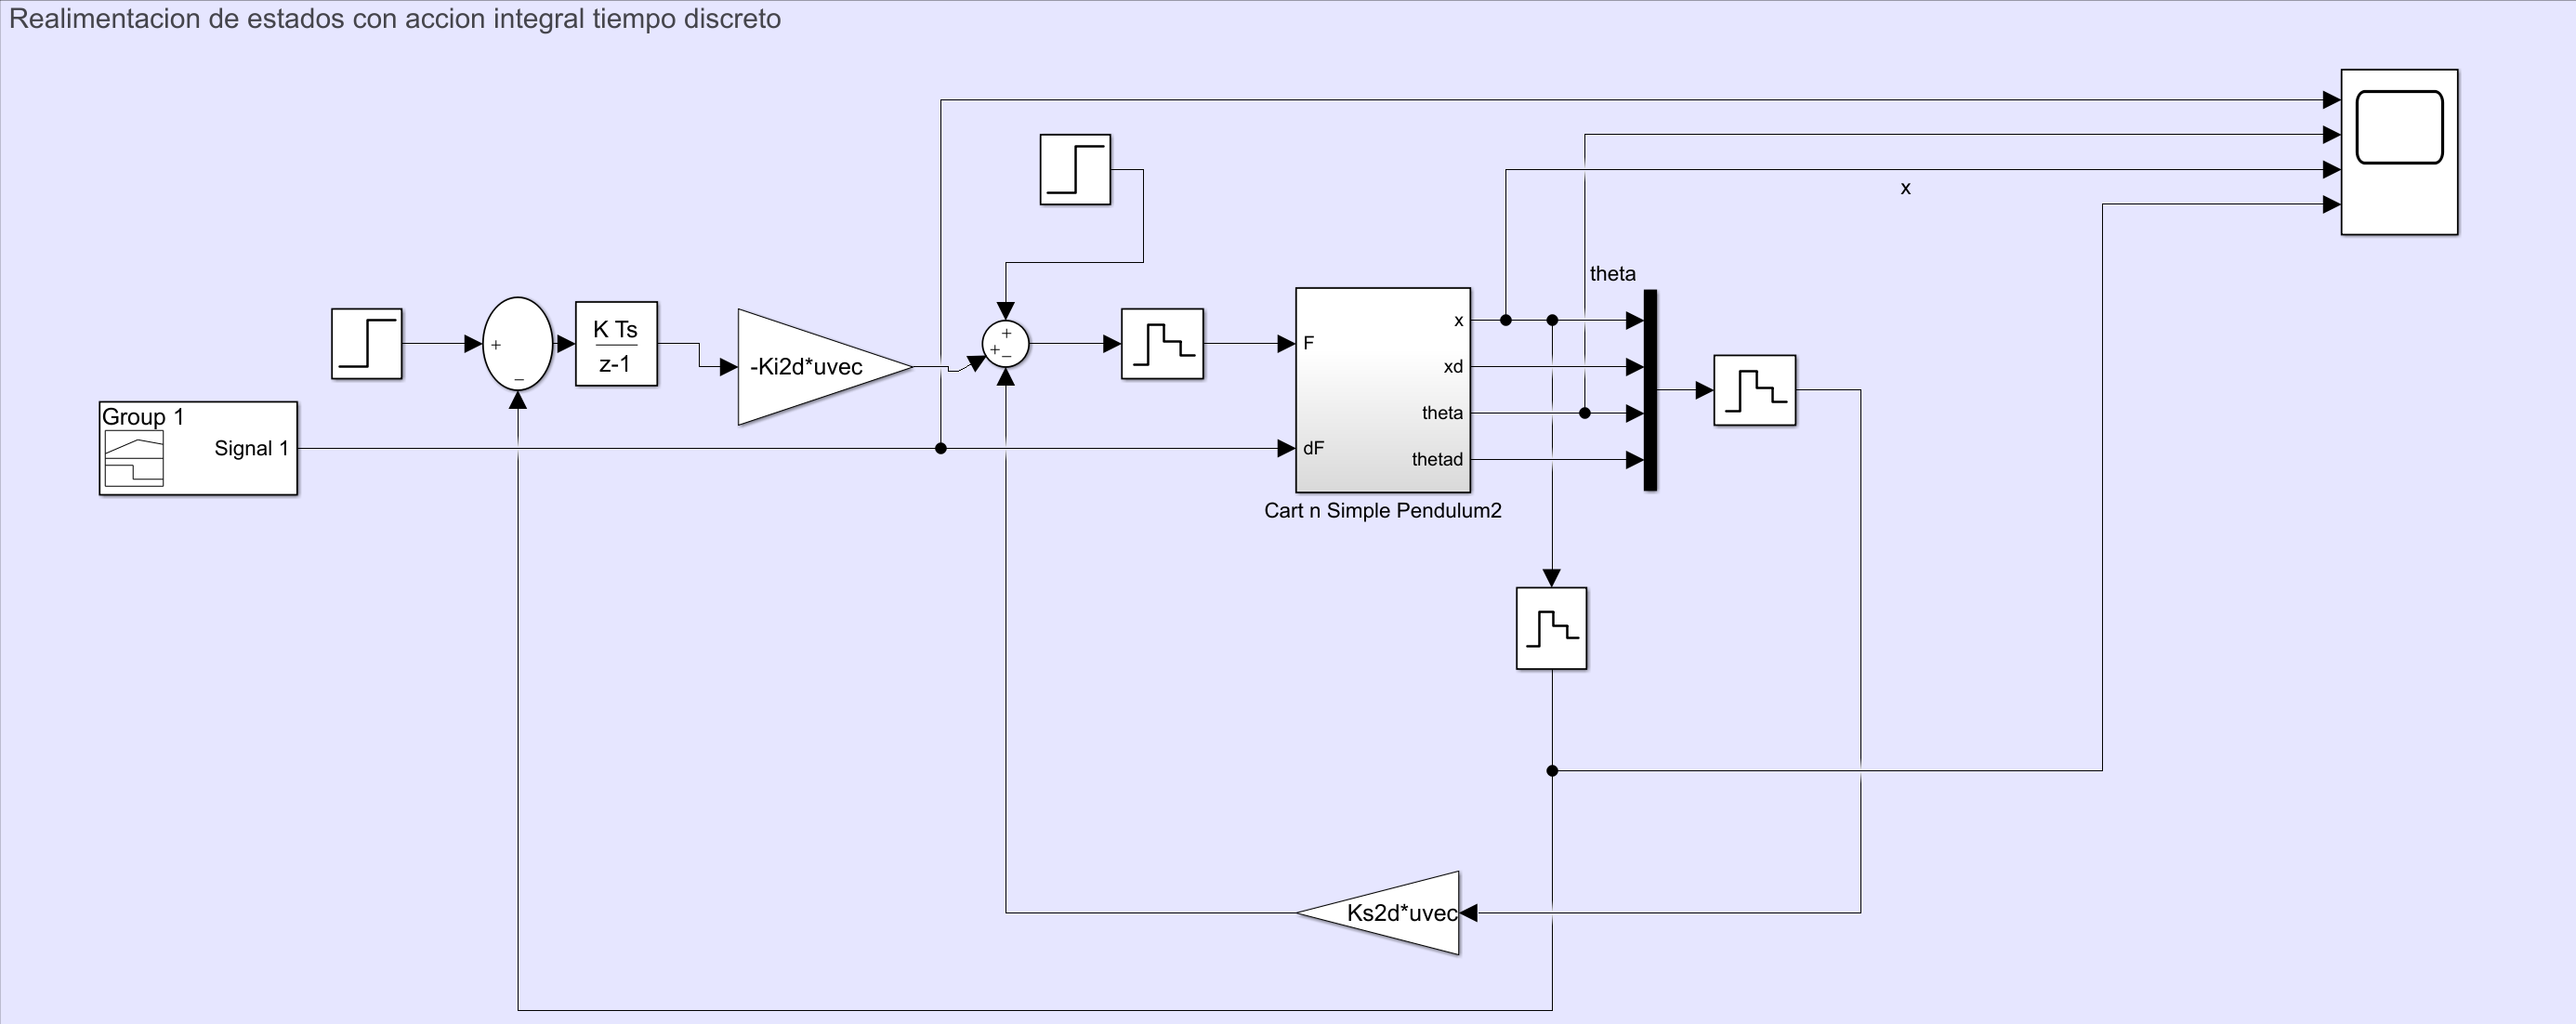
\includegraphics[width=0.8\linewidth]{ImagenesRealimentacióndeEstados/discreteIntegralFeed}
	\caption{Control por Realimentación de estados con acción integral en tiempo discreto.}	
	\label{fig:discreteIntegralFeed}
\end{figure}

Para ubicar los polos, se utiliza \textit{lqi} (\textit{lqr} con acción integral), dándole poca penalización en la matriz Q a la posición y a la velocidad del carrito, y mucha al ángulo en el que se encuentra. Además, se selecciona un tiempo de muestreo de 50 ms.

Conservando las entradas del caso anterior, se muestran las salidas del sistema continuo y su discretización en la Figura (\ref{fig:discreteIntegralFeedOut}).
\begin{figure}[H]
	\centering
	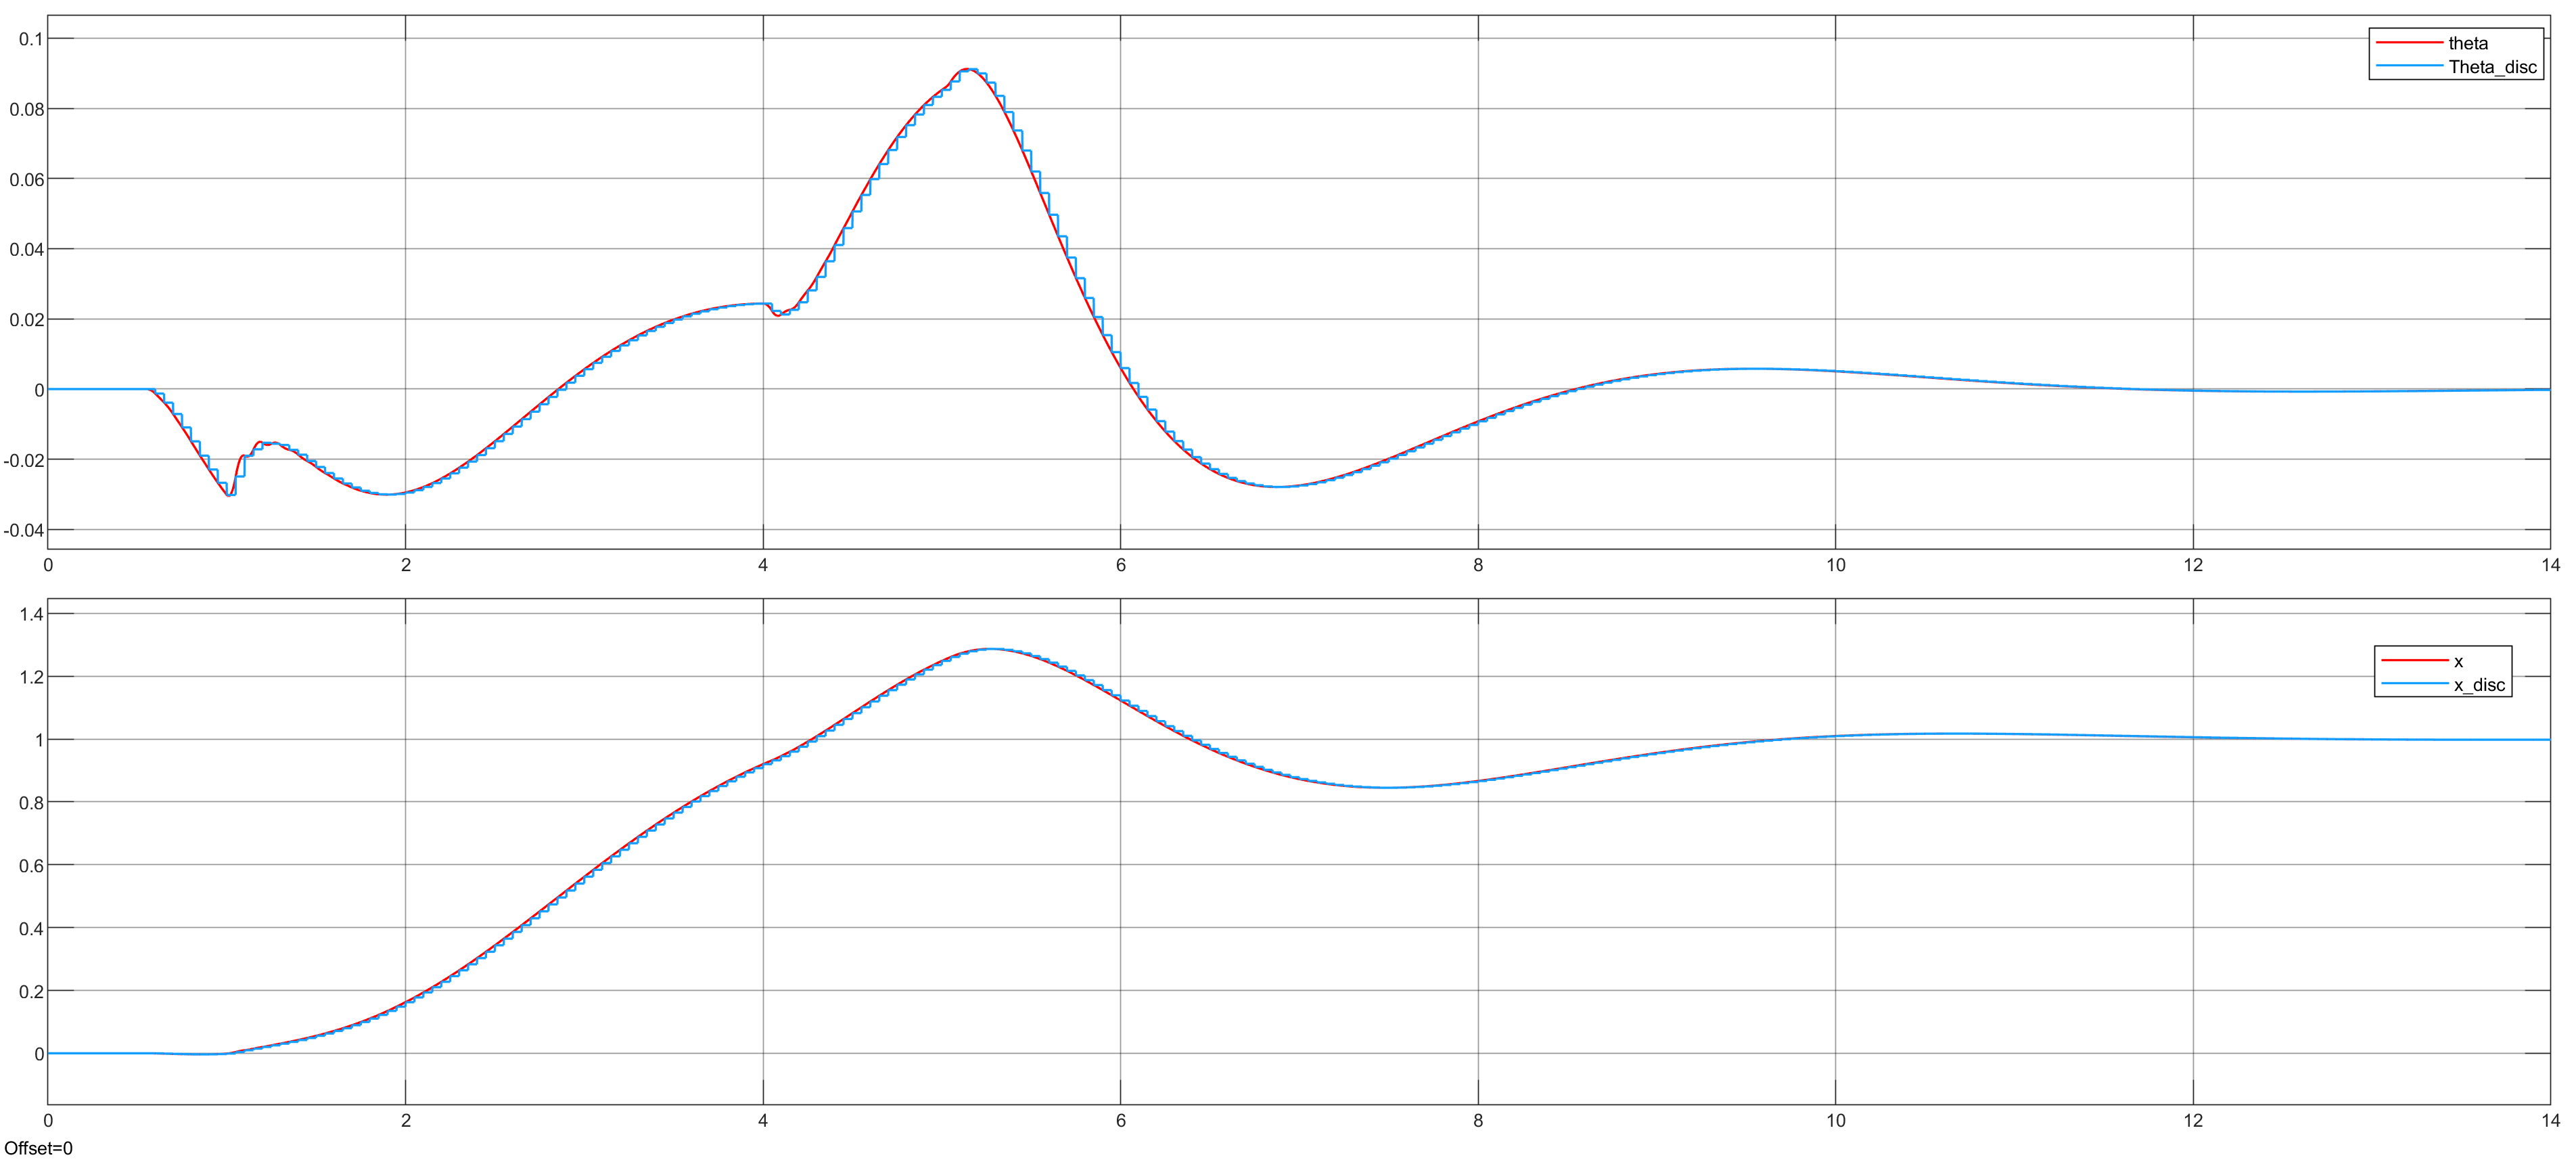
\includegraphics[width=0.8\linewidth]{ImagenesRealimentacióndeEstados/discreteIntegralFeedOut}
	\caption{Salidas del Control por Realimentación de estados con acción integral en tiempo discreto.}	
	\label{fig:discreteIntegralFeedOut}
\end{figure}

Se puede observar que en este caso el funcionamiento del sistema continua siendo correcto.
%\end{document}